\documentclass[12pt,a4paper]{article}
\usepackage[utf8x]{inputenc}
\usepackage{float}
\usepackage{graphicx}
\usepackage{setspace}
\usepackage{listings}
\usepackage{xcolor}
\usepackage{pdflscape}
\usepackage{fancyhdr}
\usepackage{caption}
\usepackage{enumitem}
\usepackage{listings}
\newcommand{\leftimage}{informatika.jpg}
\newcommand{\rightimage}{ehu.png}
\definecolor{darkgreen}{rgb}{0,0.5,0}
\definecolor{lightgray}{rgb}{0.95,0.95,0.95}
\definecolor{gray}{rgb}{0.65,0.65,0.65}
\lstset{language=C,
	basicstyle=\scriptsize\ttfamily,
	inputencoding=utf8,
	keywordstyle=\color{darkgreen}\bfseries,
	morekeywords={punto, hiruki},
	identifierstyle=\color{blue},
	commentstyle=\color{gray}, 
	stringstyle=\ttfamily,
	showstringspaces=false,
	tabsize=2,
	backgroundcolor=\color{lightgray},
		literate={
		{á}{{\'a}}1
		{é}{{\'e}}1
		{í}{{\'i}}1
		{ó}{{\'o}}1
		{ú}{{\'u}}1
		{ñ}{{\~n}}1
		{Á}{{\'A}}1
		{É}{{\'E}}1
		{Í}{{\'I}}1
		{Ó}{{\'O}}1
		{Ú}{{\'U}}1
		{Ñ}{{\~N}}1
		}}

\pagestyle{fancy}

\fancyhead[L]{\hspace*{-3.5cm}\includegraphics[height=2cm]{\leftimage}}

\fancyhead[R]{\hspace*{11cm}\includegraphics[height=2cm]{\rightimage}}
 
\setlength{\headheight}{60.50554pt}
\renewcommand{\headrulewidth}{0pt}

\begin{document}
\renewcommand*\contentsname{Índice}
\begin{titlepage}
	\begin{center}
	\vspace*{-4cm}	
       \begin{minipage}{\textwidth}
	   \centering
	   
\includegraphics[width=100mm]{ehu.jpg}
	   \vspace*{4cm}
       \end{minipage}
       \vspace*{0.5cm}

	

       \textbf{Ingeniería Informática}\\
       \textbf{UPV/EHU}\\

       \vspace{0.5cm}
        Documentación de Gráficos por Computador.
            
       \vspace{1.5cm}

       \textbf{Mikel Molina}

       \vfill 
            
       
            
       \vspace{0.8cm}
     
            
       Gráficos por Computador\\
       23 de septiembre de 2023 
   \end{center}
            
\end{titlepage}
\tableofcontents
\clearpage
\section{Objetivos de la aplicación.}
El objetivo de la primera entrega de la aplicación es simple: Debe dibujar triángulos con una textura que se le pasa al programa. Las dimensiones y puntos del triángulo las pasará el usuario a través de un fichero. Sin embargo, el fichero debe seguir un formato concreto: cada línea contendrá un triángulo, y antes de escribir los puntos, se debe poner una "t" por delante. Así pues, cada punto del triángulo se escribirá de la siguiente forma:

$$
t\ x_1\  y_1\ z_1\ u_1\ v_1\ x_2\ y_2\ z_2\ u_2\ v_2\ x_3\ y_3\ z_3\ u_3\ v_3
$$
Donde $x_i\ y_i\ z_i\ u_i\ v_i$ son los puntos correspondientes al vértice i-ésimo del triángulo. La aplicación tenía que encargarse de dibujar el interior de los triángulos, para ello hemos hecho uso de rectas. Más adelante se explicará el método usado para lograrlo. 
\section{Interacción con el/la usuario/a}
Las teclas disponibles son de momento limitadas, tan solo se han implementado tres teclas:
\begin{enumerate}
	\item La tecla enter sirve para que el programa muestre el siguiente triángulo en el fichero entregado.
	\item La tecla "l" sirve para cambiar a un triángulo que no enseña texturas, éste ya estaba antes de empezar con el proyecto.
	\item La tecla "f" sirve para cambiar el fichero de entrada al que deseemos nosotros.
\end{enumerate}
\section{Herramientas utilizadas.}
Para llevar a cabo la primera entrega del proyecto, hemos hecho uso de GLUT (OpenGL Utility Toolkit), una librería que contiene utilidades de OpenGL, pero más manejable para un programador que se esté iniciando. Perfecto para hacer este tipo de proyectos, en los que la tarea es relativamente simple. Como esta librería se encuentra en C, el programa está escrito en este lenguaje.
\begin{figure}[H]
	\centering
\includegraphics[scale = 0.5]{opengl.png}
\end{figure}
\section{Uso de la aplicación}
El programa se puede ejecutar desde una interfaz gráfica, pero es recomendado ejecutarlo desde el terminal de linux. Esto es porque la aplicación, una vez ejecutada, leerá de un fichero predeterminado, pero tenemos la capacidad de cambiarlo, y ofrecerle uno que nosotros queramos. Éste es un ejemplo de cómo se debe usar la aplicación correctamente:

\begin{enumerate}
	\item Llamamos la aplicación desde un terminal de cualquier distribución de \textbf{Linux}.\\
	\vspace{3mm}
	\begin{minipage}{\linewidth}
		\centering
		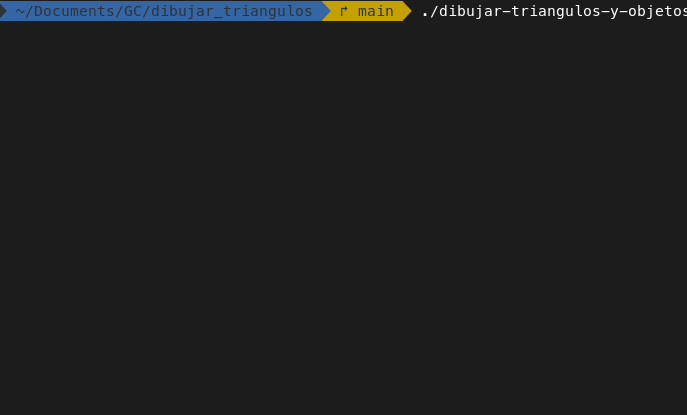
\includegraphics[scale=0.5]{llamada.png}
	\end{minipage}
	
	\item Si deseamos cambiar el fichero predeterminado, pulsamos la tecla "f" y escogemos el fichero que queramos.
	
	\begin{minipage}{\linewidth}
		\centering
		\includegraphics[scale=0.5]{cambiar_fichero.png}
	\end{minipage}
	
	\item El fichero debe seguir estrictamente este formato:
	
	\begin{minipage}{\linewidth}
		\centering
		\includegraphics[scale=0.25]{formato.png}
		\captionof{figure}{Nótese que cada línea contiene un triángulo, tal y como hemos dicho en la introducción.}
	\end{minipage}
\end{enumerate}
Por último, si deseamos cambiar la imagen del programa, hay que tener en cuenta que para ello deberemos cambiar el formato de la imagen a ppm (Portabol Pixmab). Éste formato representa los valores RGB de cada píxel mediante números que van del 0 al 255.
\section{Código C}
A continuación tenemos el código implementeado para que el programa funcionase. Como veremos, se ha dividido en varias funciones para facilitar el entendimiento, con la falta de eficiencia que ello implica. Ésta es la función principal que debíamos cambiar.
\begin{lstlisting}
	void dibujar_triangulo(triobj *optr, int i)
	{
		hiruki *tptr;
		punto *pgoiptr, *pbeheptr, *perdiptr;
		punto *pgoiptr2, *pbeheptr2, *perdiptr2;
		punto corte1, corte2;
		int start1, star2;
		float t = 1, s = 1, q = 1;
		float decremento_t = 1, decremento_s = 1, decremento_q = 1;
		float c1x, c1z, c1u, c1v, c2x, c2z, c2u, c2v;
		int linea;
		float cambio1, cambio1z, cambio1u, cambio1v, cambio2, cambio2z, 
		cambio2u, cambio2v;
		punto p1, p2, p3;
		
		if (i >= optr->num_triangles)
		return;
		tptr = optr->triptr + i;
		mxp(&p1, optr->mptr->m, tptr->p1);
		mxp(&p2, optr->mptr->m, tptr->p2);
		mxp(&p3, optr->mptr->m, tptr->p3);
		if (lineak == 1)
		{
			glBegin(GL_POLYGON);
			glVertex3d(p1.x, p1.y, p1.z);
			glVertex3d(p2.x, p2.y, p2.z);
			glVertex3d(p3.x, p3.y, p3.z);
			glEnd();
			return;
		}
		
		//Encontramos el punto máximo, mínimo, y medio del triángulo.
		
		encontrar_max_min(tptr, &pgoiptr, &perdiptr, &pbeheptr);
		
		// Llamada a función rellenar triángulo.
		
		rellenar_triangulo(pgoiptr, perdiptr, pbeheptr);
		
	}
\end{lstlisting}
Como podemos ver, solo hemos puesto dos funciones, veamos de cerca ambas:
\begin{lstlisting}
	void encontrar_max_min(hiruki *tptr, punto **pgoiptr, punto **perdiptr, 
	punto **pbeheptr)
	{
		if (tptr->p1.y > tptr->p2.y)
		{
			if (tptr->p1.y > tptr->p3.y)
			{
				*pgoiptr = &(tptr->p1);
				if (tptr->p2.y > tptr->p3.y)
				{
					*perdiptr = &(tptr->p2);
					*pbeheptr = &(tptr->p3);
				}
				else
				{
					*perdiptr = &(tptr->p3);
					*pbeheptr = &(tptr->p2);
				}
			}
			else
			{
				*pgoiptr = &(tptr->p3);
				*perdiptr = &(tptr->p1);
				*pbeheptr = &(tptr->p2);
			}
		}
		else if (tptr->p2.y > tptr->p3.y)
		{
			*pgoiptr = &(tptr->p2);
			*pbeheptr = &(tptr->p1);
			*perdiptr = &(tptr->p3);
		}
		else
		{
			*pgoiptr = &(tptr->p3);
			*pbeheptr = &(tptr->p1);
			*perdiptr = &(tptr->p2);
		}
	}
\end{lstlisting}
encontrar max min busca, dado un triplete de puntos, el punto con mayor valor de $y$, el número con menor de $y$, y el número intermedio de $y$. Cada punto al que le pertenezca dicha $y$ será guardado en el punto que le corresponde pasado por la función.
\begin{lstlisting}
	content...
\end{lstlisting}
\end{document}
